%
% Grizzards printable manual
%
% This needs a lot of work yet.
%
% If you're a human, skip to "\mainmatter" to skip over the preamble.
%
\documentclass[10pt,twocolumn,openany,article]{memoir}

\setstocksize{9in}{6in}
\settrimmedsize{\stockheight}{\dimexpr 6in-15mm}{*}

\setlrmarginsandblock{.5cm}{1.5cm}{*}
\setulmarginsandblock{1.5cm}{*}{1}
\checkandfixthelayout


%% TV Standard

\ifdefined\TVNTSC
\newcommand\TV{NTSC}
\newcommand\REGION{US, Canada, Mexico, Brazil, and Japan}
\else
\ifdefined\TVPAL
\newcommand\TV{PAL}
\newcommand\REGION{UK and Europe (except France)}
\else
\ifdefined\TVSECAM
\newcommand\TV{SECAM}
\newcommand\REGION{France, Russia, Africa}
\else
\error{Must define a TV standard}
\fi
\fi
\fi


\usepackage[utf8]{inputenc}
\usepackage{babel}
\usepackage{microtype}
\usepackage{graphicx}
\usepackage{pdfpages}
\tolerance=1
\emergencystretch=\maxdimen
%\usepackage{tgtermes}
\usepackage{hyperref}
\usepackage{xcolor}
\hypersetup{
    colorlinks,
    linkcolor={red!50!black},
    citecolor={blue!50!black},
    urlcolor={blue!80!black},
    pdftitle={Grizzards \ifdefined\DEMO{ Demo }\fi Manual for \TV},
    pdfsubject={Grizzards videogame for the Atari 2600},
    pdfauthor={Bruce-Robert Pocock}%,
%    pdfkeywords={Your PDF keywords}
  }
\usepackage{caption}
\captionsetup{labelformat=empty}
\usepackage[protrusion=true,expansion=true]{microtype}
\fontfamily{pnc}
\chapterstyle{komalike}

\checkandfixthelayout

\title{Grizzards \ifdefined\DEMO Demo \fi Player's Guide}
\author{Bruce-Robert Pocock}


%%% BEGIN DOCUMENT

\begin{document}
\frontmatter
%%%\let\cleardoublepage\clearpage
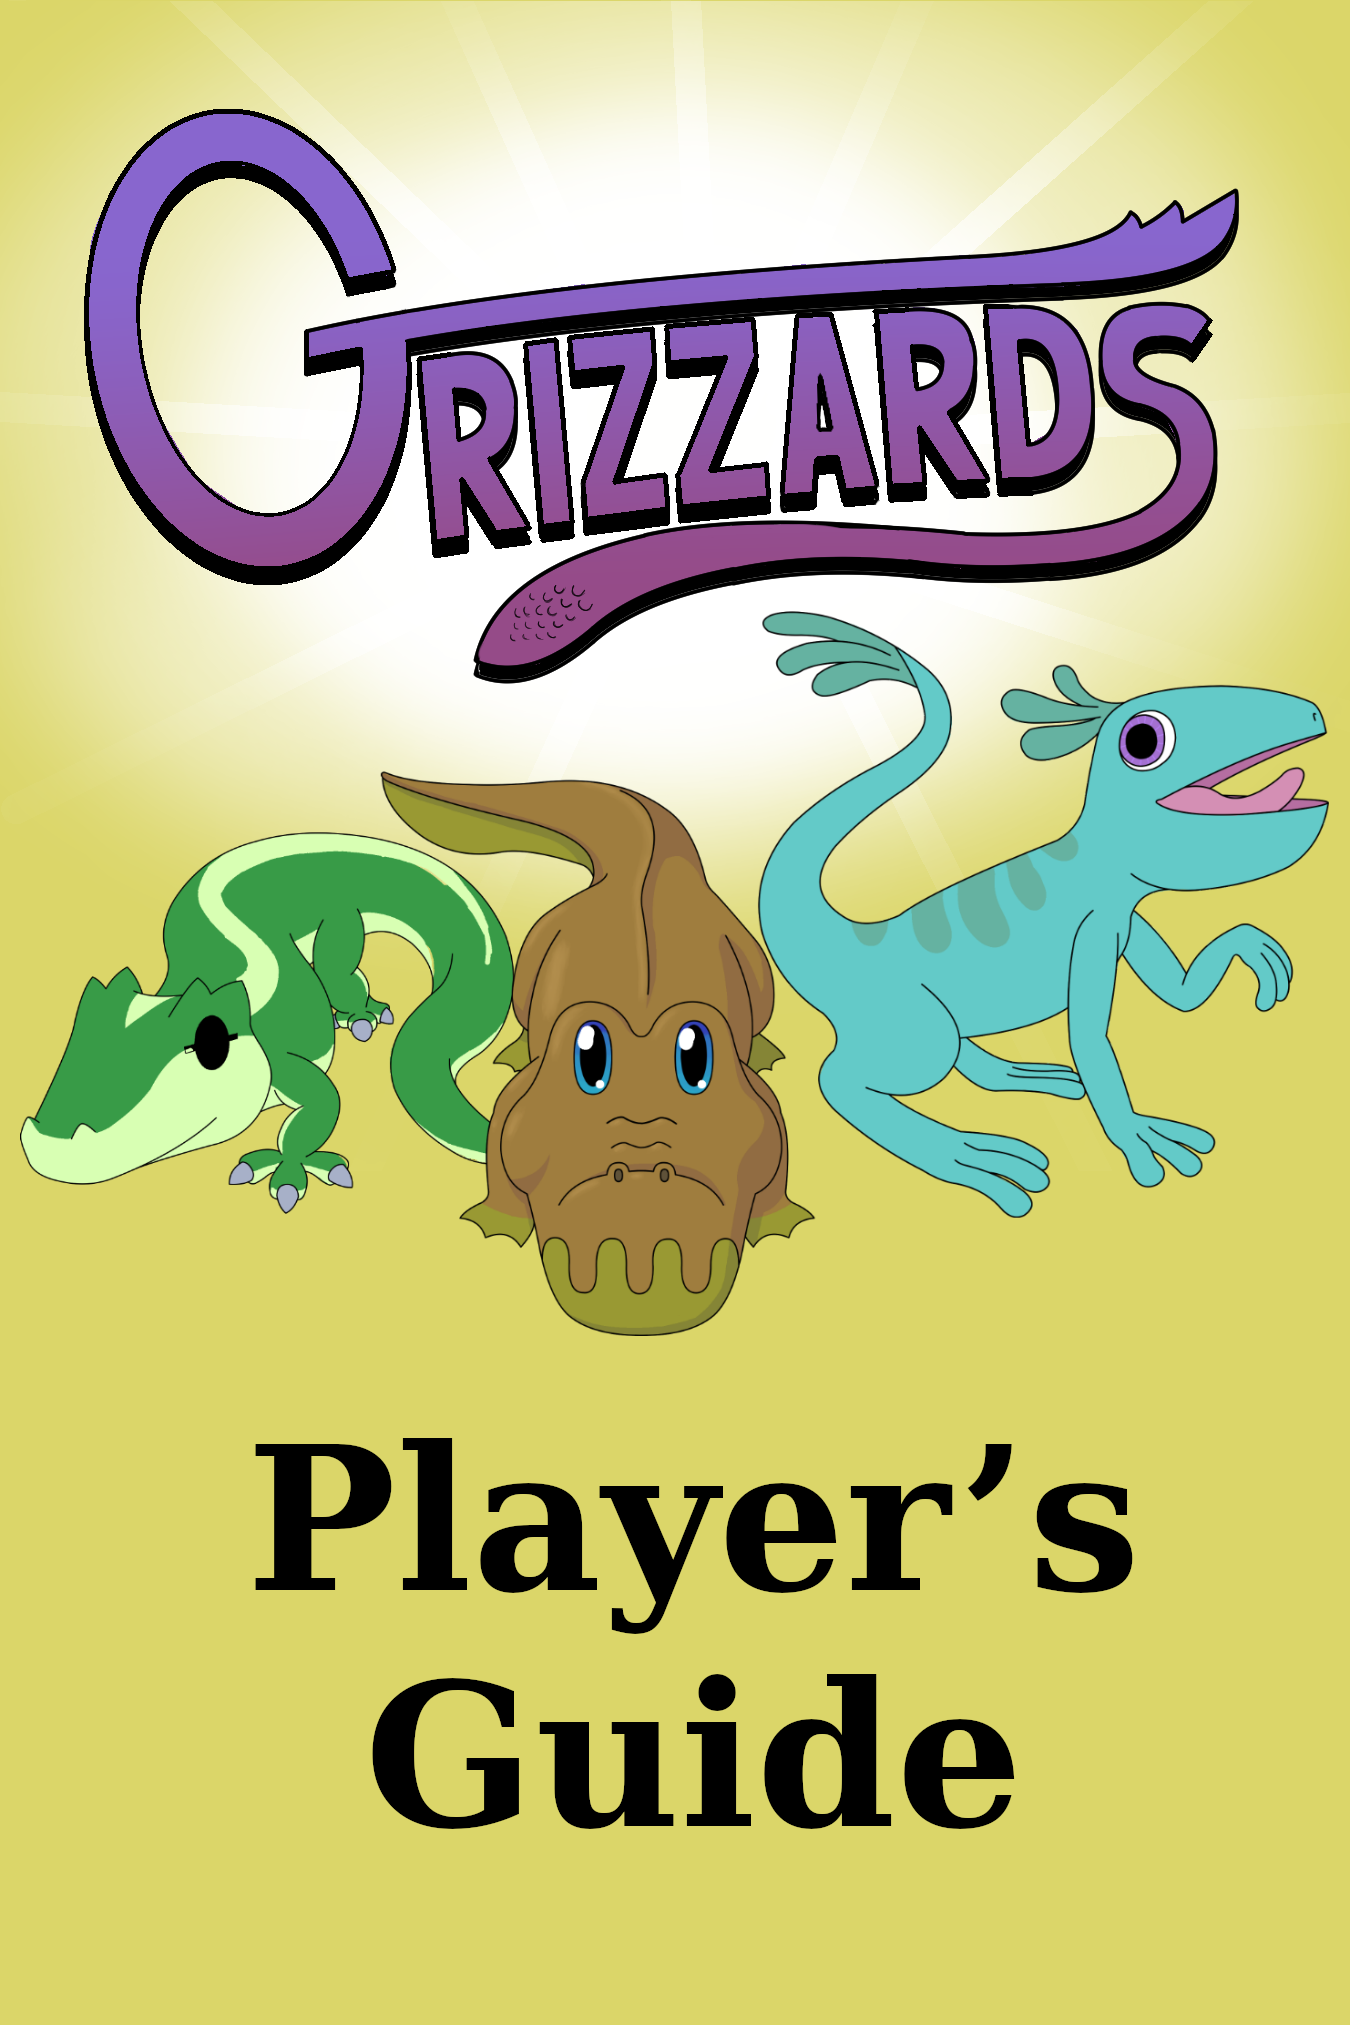
\includepdf{../Manual/Cover.png}

% \clearpage

% \maketitle

\thispagestyle{empty}

\twocolumn[

\chapter*{Introduction}\label{Introduction}

The  land of  Syrex  is  a dangerous  place.  Fierce  monsters roam  the
countryside. But luckily for you, you're a Grizzard handler!

Train your Grizzard to  use a variety of moves to  take on the monsters.
Discover new kinds  of Grizzards with new capabilities.  Can you conquer
all the monsters of Syrex?

\bigskip

In the \textit{Grizzards}  videogame, you'll roam the land  looking for monsters.
Monsters may  surprise you as  you travel, or  you may see  them coming.
When faced  with terrifying beasts,  you'll direct your Grizzard  to use
its moves to defend you and attack the monsters.

\vspace{1in}\vfill

This is the \textit{Grizzards} \ifdefined\DEMO Demo \fi Player's Guide

Copyright \copyright{} 2021, Bruce-Robert Pocock

\bigskip

This  version is  for systems  in \REGION{}  using the  \TV{} television
standard. For Atari  Video Computer System CX-2600  (or Sears Tele-Games
Video  Arcade or  Atari 7800  ProSystem) with  AtariVox (or  MemCard, or
SaveKey) device.

\bigskip

This videogame software was not created, published, or licensed by Atari
or its successors.

\ifdefined\DEMO
\bigskip

This manual describes  a DEMO version of the game.  The full version may
be different.
\fi

]

\let\cleardoublepage\clearpage

\mainmatter

\tableofcontents

\chapter{Setting Up}\label{Setting Up}

To play \textit{Grizzards}, you will need:

\begin{itemize}
\item An Atari  console: the Atari Video Computer  System CX-2600, Sears
  Tele-Games  Video Arcade,  Atari  2600jr game  system,  or Atari  7800
  ProSystem
\item A TV or video display
\item A joystick controller
\item A  memory device: an  AtariVox device with (optional)  speakers or
  headphones, or a MemCard or SaveKey device.

  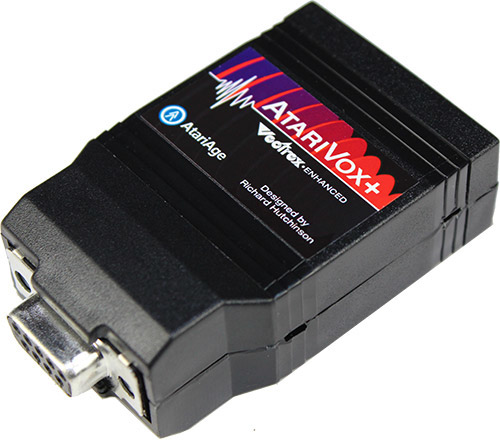
\includegraphics[width=.4\columnwidth]{../Manual/AtariVox.jpeg}
  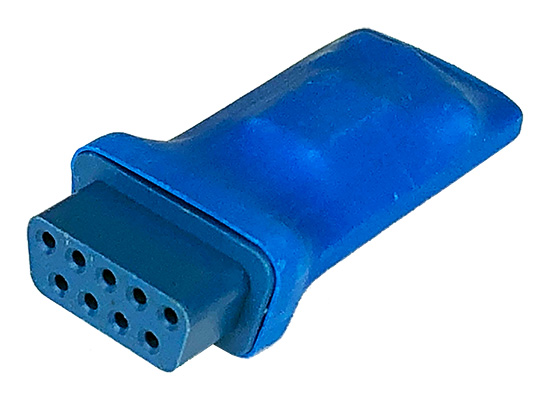
\includegraphics[width=.4\columnwidth]{../Manual/SaveKey.jpeg}

\item The \textit{Grizzards} game cartridge
\end{itemize}


Set  up your  Video  Computer  System with  your  TV  or video  display.
Connect a  joystick controller to  the \emph{left} controller  port, and
the memory device to the \emph{right} controller port. Make certain that
the  Power  switch   is  in  the  Off  position   when  connecting  your
memory device.

Finally, insert  the \textit{Grizzards}  game cartridge (with  the label
facing up) into the cartridge slot, and turn the Power On.

\begin{figure}[h]
  \begin{center}
    \includegraphics[width=\columnwidth]{../Manual/Atari-2600-Wood-4Sw-Set.png}
  \end{center}
\end{figure}


\vfill

\chapter{How To Play}

\section{Console Controls}

\ifdefined\TVSECAM
\else

\subsection{Color/B\&W Switch (Pause)}

On an  Atari 2600  (or Sears Arcade)  you can pause  the game  using the
Color/B\&W Switch. Push the Color/B\&W switch into the Color position to
play, or the B\&W position to pause the game.

On the Atari  7800, press the Pause  button once to pause  the game, and
again to resume playing.

\fi

\subsection{Game Select}

When viewing  the Title Screen,  you can use  the Game Select  switch to
choose the Slot you wish to use to save your progress.

While you are  playing the game, you  can use the Game  Select switch to
review   your  Grizzard's   statistics   from  the   Combat  screen   or
a Grizzard Depot.

On the Map screen, the Game Select switch has no effect.

\subsection{Game Reset}

When viewing  the Select  Slot screen,  press the  Game Reset  switch to
begin playing the game.

While you are  playing the game, press the Game  Reset switch to abandon
your progress and return to the Title Screen. You will lose any progress
since the last time you visited a Grizzard Depot.

\subsection{Difficulty Switches}

You cannot delete a game in progress unless both Difficulty Switches are
in the  ``A'' (Advanced or Expert)  position. To protect your  game from
being deleted,  set either one of  the Difficulty Switches to  the ``B''
(Beginner or Novice) position.

\ifdefined\TVSECAM

The Left Difficulty Switch  can be used to pause game  play. When in the
``A'' (Advanced  or Expert) position, you  will not be able  to continue
playing  until  you  toggle  the   switch  to  the  ``B''  (Beginner  or
Novice) position.

You cannot delete a game in progress unless both Difficulty Switches are
in the ``A'' (Advanced or Expert) position.

\else

This  game does  not  make  use of  the  Difficulty  Switches while  you
are playing. 

\fi

\section{Start a Game}

\begin{center}
  \includegraphics[width=\columnwidth]{../Manual/TitleAquax\TV.png}
\end{center}

Once your  console is set  up and everything  is connected, turn  on the
Power  switch. You'll  see  the  title screen  appear.  If  you have  an
AtariVox device, you'll also hear the title spoken.


\begin{center}
  \includegraphics[width=\columnwidth]{../Manual/SelectSlot\TV.png}
\end{center}

Press  the Game  Select switch  or  Fire button  to move  to the  Select
Slot screen.

Press the  Game Select  switch or  move the joystick  left and  right to
choose  a memory  slot\footnote{Technical Note:  The Slot  number chosen
  here  is  relative   to  the  three  save  game  slots   used  by  the
  \textit{Grizzards} game program. Each save game slot actually occupies
  4 blocks  on your memory  device.} for your  game. There are  3 memory
slots  possible. Press  Game  Select  or the  joystick  again to  rotate
through them. If someone has already begun to play \textit{Grizzards} in
a certain slot, your screen will  show ``\texttt{RESUME}.'' If a slot is
empty, you'll see ``\texttt{BEGIN}'' instead.

\ifdefined\DEMO
\skip
This  demo  saves your  progress  in  the  ``scratchpad'' area  of  your
memory  device.  It's possible  that  other  games might  overwrite  and
destroy your saved progress. This is  just because it's a demo, and does
not have a private area reserved for it yet.
\skip
\fi

When you have selected the slot you want to begin (or resume), press the
Game Reset switch or Fire button to start.

\section{Roaming The World}

The   World   Map   screen   shows   your   current   score   (initially
\texttt{000000}) at  the top of the  screen. In the map  display, you'll
see the  current area in which  you are traveling. Guide  yourself using
the joystick controller.

\begin{center}
  \includegraphics[width=\columnwidth]{../Manual/Map\TV.png}
\end{center}

As   you  travel,   you   may  encounter   monsters,\ifdefined\DEMO\else
Grizzards,  \fi  Grizzard Depots,  other  people,  signposts, or  doors.
To interact with them, simply walk into them.

A  monster,  or group  of  monsters,  look  like this:

\begin{center}
  \includegraphics[width=1in]{../Manual/Monster\TV.png}
\end{center}

Sometimes these  monsters may sneak  up on  you and attack!  Other times
you'll see  them waiting for you  and can avoid  them --- or walk  up to
them when you're ready to face them.

A Grizzard Depot looks like this:

\begin{center}
  \includegraphics[width=1in]{../Manual/Depot\TV.png}
\end{center}

\ifdefined\DEMO
In this demo,  you will have one Grizzard companion,  Aquax. In the full
game, you  may encounter other Grizzards  that you can convince  to join
your party.

\else

You may also  encounter Grizzards in the world that  you can convince to
join your party. A wild Grizzard looks like this:

***

At a  Grizzard Depot, you'll have  the option to swap  Grizzards in your
party,  with up  to  30 total  Grizzards saved  in  your memory  device.
Each Grizzard may have its own moves and skill scores.

\fi

To  review the  statistics  of your  current  Grizzard companion,  press
Game Select.

A door looks like this:

\begin{center}
  \includegraphics[width=1in]{../Manual/Door\TV.png}
\end{center}

A signpost looks like this:

\begin{center}
  \includegraphics[width=1in]{../Manual/Signpost\TV.png}
\end{center}

A person looks like this:

\begin{center}
  \includegraphics[width=1in]{../Manual/Person\TV.png}
\end{center}

\section{Grizzard Depots}

To \ifdefined\DEMO\else  swap which  Grizzard you're using,  or to  \fi heal
your current Grizzard partner, you'll need to find a Grizzard Depot.

\includegraphics[width=\columnwidth]{../Manual/DepotScreenshot\TV.png}

Touch the Grizzard Depot on the map screen to enter it.

Your progress will \emph{immediately} be saved to your memory device.

At  a  Grizzard  Depot  your  Grizzard partner  will  be  fully  healed.
\ifdefined\DEMO\else You  can then  use the joystick  to choose  a different
Grizzard to travel with you. \fi

Here,  you'll  see  the   word  \texttt{DEPOT},  your  current  Grizzard
companion,  and  the  number  of hours  you've  been  playing  Grizzards
(total, since you first started in this slot).

To review your Grizzard's statistics, press the Game Select switch.

\ifdefined\DEMO\else
If you  have more than one  Grizzard in your collection,  you can choose
which  Grizzard will  be  your  companion. Press  up  (forward) or  down
(backward)  on  the  joystick  controller  to  cycle  through  available
Grizzards.
\fi

When you're ready to return to your adventure, press the Fire button.


\section{Battling Monsters}

Monsters plague the world of Syrex. If you're caught by monsters without
a Grizzard partner, they're sure to eat you alive! Luckily your Grizzard
partner  will  defend  you  from  them,  and  monsters  will  attack  it
before you.

When you encounter monsters, you'll  see the Combat display.

\begin{figure}
  \includegraphics[width=\columnwidth]{../Manual/CombatScreen\TV.png}
  \caption{The Combat screen}
\end{figure}

Monsters may  travel in  groups, so  you may see  more than  one monster
facing you.

The  long bar  beneath your  Grizzard represents  its health.  If it  is
reduced to zero, your adventure will be over.

Using the joystick controller, you can  choose from among the moves that
your Grizzard knows how to perform. Press  up and down to select a move.
If your Grizzard knows  how to perform a move, it  will appear in color.
If your Grizzard does not yet know how to perform a move, it will appear
in black.

Most  Moves will  target one  monster  that you're  facing. (Some  Moves
instead affect yourself.) Press left or right on the joystick controller
to select a target if you're facing multiple monsters.

When you  see the selection  you want, press  the Fire button.  You must
select a move that your Grizzard knows how to perform.

To review the statistics of your Grizzard, press Game Select.

\begin{figure}
  \includegraphics[width=\columnwidth]{../Manual/StatsScreenshot\TV.png}
  \caption{Viewing your Grizzard's statistics}
\end{figure}

\subsection{Executing a Move}

It's possible for a move to miss its target. If that happens, you'll see
\texttt{MISSED} appear briefly.

After a move  has been executed, the creature targeted  by that move may
be injured (lose hit points) or  have its statistics changed. Changes to
statistics  are temporary  and last  only  the duration  of one  battle.
After the battle,  your Grizzard's statistics (or those  of any monsters
you failed to defeat) will return to normal.

If  you Grizzard  loses hit  points, the  bar below  your Grizzard  will
reduce in  length. When your Grizzard  is nearly out of  hit points, the
bar will change to a red color to draw attention to that fact.

If your  Grizzard is defeated, the  monsters will surely eat  you alive.
Your adventure  will end there, and  you'll return to the  title screen.
Don't worry, though;  you can continue from the last  Grizzard Depot you
visited by  resuming your  game's saved progress.  Just choose  the same
game slot and resume and try again.

If you  defeat all of  the monsters, victory  is yours! Your  score will
increase, and you'll return to the World Map screen victorious.

You  may choose  to run  away from  a fight,  but the  monsters will  be
immediately healed and may still come after you.

\subsection{Grizzard Learning}

Your  Grizzard companion  may  learn from  opposing  Monsters. This  can
result  in your  Grizzard  increasing  its Attack  or  Defend score,  or
learning a Move that a monster has just performed.

Your Grizzard  can only  learn certain moves.  Moves that  your Grizzard
might be able to  perform, but does not yet know how  to, will appear in
black on the Combat display.

\subsection{Statistics}

You can also  press the Game Select switch during  combat to review your
Grizzard's statistics. Each Grizzard companion has a few statistics:

\begin{description}
  
\item[\texttt{ATK}] is the Grizzard's  \emph{attack} rating. This is the
  amount  of damage  that  your  Grizzard can  do  when it  successfully
  attacks a monster. Some Moves cause more damage than others, though.
  
\item[\texttt{DEF}] is the Grizzard's  \emph{defend} rating. This is how
  likely your Grizzard is to avoid being hurt by a monster's Move.

\item[\texttt{HP}]  is  the  Grizzard's  \emph{hit  points}  or  health.
  When  monsters hit  your Grizzard,  this  value will  decrease. If  it
  reaches zero, your game is over.

\item[\texttt{MAX}]  is   the  Grizzard's  \emph{maximum   hit  points}.
  Your Grizzard can gain more hit points up to this amount.
  
\end{itemize}

Each of  these statistics can  be raised up to  a maximum of  99 points.
They may go up a bit after each monster that you defeat.

Your  Grizzard may  also  be  subject to  one  or  more Status  Effects.
These  will  alter your  Grizzard's  status  temporarily (only  for  the
duration of  one battle).


\subsection{Status Effects}

A move can affect its target with Status Effects. There are six possible
Status Effects that can influence a creature:

\begin{description}
\item[\texttt{SLEEP}] A creature which has gone to sleep can not move on
  their turn. There is a 50\% chance of waking on each turn.
\item[\texttt{ATK UP}] A  creature with Attack Up has  its normal attack
  score doubled.
\item[\texttt{ATK DN}] A creature with Attack Down has its normal attack
  score halved.
\item[\texttt{DEF UP}] A  creature with Defend Up has  its normal defend
  score doubled.
\item[\texttt{DEF DN}] A creature with Defend Down has its normal defend
  score halved.
\item[\texttt{MUDDLE}] A creature which has been Muddled will choose its
  moves at random. There is a 50\% chance of clearing its mind on each turn.
\end{description}

\subsection{Scoring}

When you  defeat a monster, you'll  earn points. The number  of points
you earn will increase as you defeat more difficult monsters.

Your score begins at \texttt{000000} when you start your adventure.

\section{Game Over}

If  you fail  in your  mission,  your game  is over.  However, you  have
another chance to continue.

\includegraphics[width=\columnwidth]{../Manual/GameOver\TV.png}

When you continue, it'll  be just as if you'd never  failed in the first
place. However, you'll start over from  the last Grizzard Depot that you
had visited. If you fail before visiting a Grizzard Depot, you'll return
to the original starting point.

Just  choose   your  game   slot  from  the   Title  Screen   to  resume
your adventure.

\section{Winning the Campaign}\label{Winning the Campaign}

\ifdefined\DEMO

It is not possible to ``win'' the demo version of this game. You'll have
to wait for the full game to be released!

\else

If  you  defeat  all of  the  main  monsters  in  the game,  you'll  see
a fireworks  show to let  you know  that you've completed  the campaign.
Your ``final'' score will appear above the fireworks display.

\fi

\section{Starting Over}\label{Starting Your Adventure Over}

When you choose a  slot with no game record in  it already, you'll begin
a new adventure.

If you want to delete your adventure  and start again, it's a little bit
tricky. This is to make sure you don't accidentally lose your progress!

From the Title Screen, press Game Select or the Fire button. Then, press
Game Select or move the joystick left  and right until the slot you want
to erase is shown.

Here's the tricky part. You'll need to:

\begin{itemize}
\item Make sure that both of the Difficulty Switches on your console
  are set to the ``A'' (Advanced or Expert) position.
\item With your joystick controller, pull down (toward you) on the
  joystick and hold down the Fire button.
\end{itemize}

The screen  will change from  saying ``\texttt{SELECT SLOT}''  to saying
``\texttt{ERASE  SLOT}.''   The  text   will  also   be  red   to  catch
your attention.

If  you're  \emph{sure}   you  want  to  erase  your   game  data,  then
\emph{without}  letting go  of the  Fire  button, move  the joystick  up
(toward  the TV).  You'll see  that the  slot changes  from ``\texttt{IN
  USE}'' to ``\texttt{VACANT}'' \emph{immediately}.

\emph{Once your  game record has been  erased, there's no way  to get it
  back, so think carefully before you erase it.}

\subsection{Protecting Your Game Record}

If  either of  your Difficulty  Switches is  in the  ``B'' (Beginner  or
Novice) position, then you can't erase  a game slot. \emph{Tip: When you
  connect your memory device, check the position of those switches.}

\ifdefined\TVSECAM
Remember,  the  Left  Difficult  Switch  is  used  to  pause  the  game.
After deleting your save game slot, return the Left Difficulty Switch to
the ``B'' position.
\fi

\clearpage

\chapter{Grizzards and Moves}

There are  30 Grizzards in  the game world,  each with their  own unique
starting attributes and sets of Moves.

\ifdefined\DEMO

In this  demo, you  can play  with only Aquax.  Other Grizzards  will be
available in the full game.

\fi

Each Grizzard is able  to learn up to 8 different  moves, in addition to
the universal move  \texttt{RUN AWAY}. It's up to you  to discover which
Moves each  Grizzard is  able to  learn.

\ifdefined\DEMO\else

Depending on which edition of  \textit{Grizzards} you have, you'll start
with  one  of  three  different Grizzard  companions.  Your  ``starter''
Grizzard will be featured on the title screen of the game.

\section{Dirtex}


\includegraphics[width=\columnwidth]{../Source/Banks/Bank00/Grizzard0-1.png}

The green Dirtex Grizzard lives in the grass. It can learn these Moves:

\begin{itemize}
\item \texttt{KICK DIRT} --- kick dirt at the enemy, causing some damage
  to them.
\item \texttt{BURY DEEP} --- try to bury the enemy, which may cause them
  to fall asleep.
\item  \texttt{DIRTY FOOT}  --- causes  some  damage and  may lower  the
  enemy's defend value.
\item \texttt{LOAMY FEAR} --- may lower the enemy's attack value.
\item \texttt{DUSTY EYES} --- may lower the enemy's defend value.
\item \texttt{FIRST  AID} ---  heals a small  amount of  health, raising
  your own hit points.
\item \texttt{SIMPLE CURE} --- heals a bit larger amount of health.
\item \texttt{COMMON CURE} --- heals even more health.
\end{itemize}

\fi

\section{Aquax}

\includegraphics[width=\columnwidth]{../Manual/Aquax\TV.png}

Aquax is a brown Grizzard which lives  in the swamps. It can learn these
Moves:

\begin{itemize}
\item  \texttt{SPLISH SPLASH}  --- splash  water at  the enemy,  causing
  some damage. 
\item \texttt{RAISE HOPE} --- may increase its own defend ability.
\item \texttt{SURE SPLASH} --- may increase its own attack ability.
\item \texttt{QUICK FOOT}  --- causes some damage and  may also decrease
  the enemy's defend ability.
\item \texttt{GREAT MOJO}  --- causes some damage and  may also decrease
  the enemy's attack ability.
\item \texttt{FIRST  AID} ---  heals a small  amount of  health, raising
  your own hit points.
\item \texttt{SIMPLE CURE} --- heals a bit larger amount of health.
\item \texttt{COMMON CURE} --- heals even more health.
\end{itemize}

\ifdefined\DEMO\else

\section{Airex}


\includegraphics[width=\columnwidth]{../Source/Banks/Bank00/Grizzard2-0.png}

Airex is a teal Grizzard which lives in the trees. It can learn these Moves:

\begin{itemize}
\item \texttt{MILD SHOCK} --- shocks  the enemy with static electricity,
  causing some damage.
\item \texttt{WIND FIGHT} --- causes a bit more damage than \texttt{MILD SHOCK}
\item \texttt{STEAL ATTACK} --- may lower the enemy's attack value.
\item \texttt{STEAL DEFEND} --- may lower the enemy's defend value.
\item \texttt{STEAL TURN} --- may put the enemy to sleep
\item \texttt{FIRST  AID} ---  heals a small  amount of  health, raising
  your own hit points.
\item \texttt{SIMPLE CURE} --- heals a bit larger amount of health.
\item \texttt{COMMON CURE} --- heals even more health.
\end{itemize}

\fi

\section{Run Away}

This Move lets you escape from a battle.

Your  Grizzard will  not be  healed if  you run  away (unless  you visit
a  Grizzard Depot);  however, the  monsters  that you  were facing  will
be healed immediately.



\chapter{Troubleshooting}

\ifdefined\DEMO

\section{Screen ``Jitters,'' freezes, or flashes blue}

These may  be signs that  a screen  (or the transition  between screens)
does not have the correct ``scan line'' count. This is a technical error
by the game's  developer (that's me!) and must be  corrected in the next
version of the game.

If you see these effects (or if you are running in Stella, if you notice
that the scan  line count is not \ifdefined\TVNTSC 262  \else 312 \fi at
all         times)         please         report         them         to
\hred{mailto:support@star-hope.org}{support@star-hope.org} so  that they
can be corrected before the game is finished.

\fi

\section{Sad Face Screen}

If you  see the Sad  Face screen,  the game is  trying to tell  you that
there is a problem.

From  here,  you can  press  the  Game Reset  switch  to  return to  the
Title Screen.

\subsection{Red Sad Face Screen}

\includegraphics[width=\columnwidth]{../Manual/RedSadFace\TV.png}

The red  sad face screen  means that your  memory device was  not found.
Turn off  your console and connect  an AtariVox, SaveKey, or  MemCard to
the right  controller port. You  may plug  in speakers or  headphones to
your AtariVox so that you can hear the game voices.

\subsection{White Sad Face Screen}

\includegraphics[width=\columnwidth]{../Manual/WhiteSadFace\TV.png}

The white sad  face screen means that the game  has encountered an error
and cannot continue. 

You  should   not  be  able   to  reach  this  screen.   Please  contact
\href{mailto:support@star-hope.org}{support@star-hope.org}           for
additional assistance.


\section{TV goes blank when saving}

Make sure your memory device is  connected. If your memory device is not
connected when the game tries to save, you may see the TV picture remain
blank while the game tries to record your progress.

\section{No voices}

Make sure  that you have  speakers plugged  in to your  AtariVox device.
When the game first starts the title screen, after a brief pause, you'll
hear the AtariVox announce the name of the game. If you don't, make sure
that  the AtariVox  is connected  and the  speakers (or  headphones) are
connected, powered on, and turned up.

Naturally,  there  are  no  voices   when  playing  with  a  MemCard  or
SaveKey device. 

\chapter{Technical Notes}

The following notes are of interest to hackers only. You don't need to
understand anything in this section to play \textit{Grizzards}.

\section{Development Tools}

The \textit{Grizzards}  source code and development  tools are available
from \\
\href{https://Star-Hope.org/games/Grizzards/}{https://Star-Hope.org/games/Grizzards/} \\
the \textit{Grizzards} web site.

\section{Game Record Slots}

There are 3  logical game slots that  you can choose from  for the game.
Each save game  slot takes up 4  blocks (256 bytes) of  storage space on
your memory  device, for a  total of 12 blocks  for all three  save game
slots. The following blocks are used:

\ifdefined\DEMO

\begin{enumerate}
\item blocks \$c0-\$c3 (addresses \$3000-\$30ff)
\item blocks \$c4-\$c7 (addresses \$3100-\$31ff)
\item blocks \$c8-\$cb (addresses \$3200-\$32ff)
\end{enumerate}

These blocks are in the Scratchpad  area. This means that other programs
might potentially disrupt or destroy your saved game record.

The  future version  of this  game will  use a  different set  of memory
blocks  that are  reserved for  its own  private use,  so this  won't be
a problem then.

\else

\begin{enumerate}
\item blocks \$5c-\$5f (addresses \$1700-\$17ff)
\item blocks \$60-\$63 (addresses \$1800-\$18ff)
\item blocks \$64-\$67 (addresses \$1900-\$19ff)
\end{enumerate}

\subsection{Registration}

\ifdefined\FIXMERegisterGameWithAtariAge

The addresses used by the Save  Game Slots are registered with AtariAge,
so they won't conflict with any other games you might play.

\else

The save game blocks used are \emph{not yet} registered with AtariAge.

\fi

\fi


\subsection{Portability}

The save game records are in the same format for all \textit{Grizzards} game
cartridges, regardless of the region for which they were saved.  This means
that you can save your progress on an NTSC type system and then continue
playing on a PAL or SECAM system, or vice-versa.

\ifdefined\DEMO

The save  game slots used by  this demo, however, are  distinct from the
ones that will be used in the final game.

\fi

\chapter*{Credits}

{\small

  The  \textit{Grizzards} videogame  software,  including its  audiovisual
components   and  this   manual,   are   copyright  \copyright{}   2021,
Bruce-Robert  Pocock.   All  Rights  are  Reserved   except  as  granted
under license.

\begin{itemize}
\item Bruce-Robert Pocock --- Programming, Manual text, In-Game Artwork,
  Sound effects
\item Zephyr Salz --- Art for manual, label, and cover; Music
\end{itemize}

\bigskip


Includes VCS  header file by  Matthew Dillon, Olaf  ``Rhialto'' Seibert,
Andrew  Davie, and  Peter H.  Froehlich. Binary  to decimal  translation
based upon  code by  Andrew Jacobs,  based upon  code by  Garth Wilsone.
``Six  Digit Score''  48 pixel  wide  display routines  as explained  on
Stella list  by Erik  Mooney and  Bradford W.  Mott. SaveKey  EEPROM and
AtariVox  speech  synthesis driver  based  upon  code by  Alex  Herbert.
Random  number  generator  by  AtariAge  forum  user  \texttt{Supercat}.
Some  math  functions  by  AtariAge  forum  user  \textt{Omega\-matrix}.
Some math functions taken from December 1984 Apple Assembly Line. ``Have
You Played  Atari Today'' jingle  by Atari Inc. transcribed  by AtariAge
Forum user \texttt{tigger\-the\-hun}. Atari 7800 console detection logic
by Darrell Spice, Jr. AtariVox  and SaveKey illustrations in this manual
are from the AtariAge store.

Special thanks  to everyone in  the Stella and AtariAge  communities for
making this game possible.

\subsection{Testers}

This section will list anyone who helps to playtest this game. ***

}


\chapter*{Publication History}

The \textit{Grizzards} videogame software has not yet been published.

It is ``alpha'' quality software.

A demo version was created in July, 2021.
\ifdefined\DEMO This manual describes that demo. \fi

\subsection{License}

You are hereby granted permission  to make use of the \textit{Grizzards}
videogame software for \emph{non-commercial personal use}.

Redistribution not for profit is allowed, but sales of this software
requires a license.

\end{document}
